\documentclass{article}
\usepackage[utf8]{inputenc}
\usepackage[a4paper, margin=3cm]{geometry}

%Text editing
\usepackage{verbatim}
\usepackage{indentfirst}

%Package for graphic expression
\usepackage{graphicx}
\usepackage{circuitikz}
\graphicspath{ {./img/} }
\usepackage{wrapfig}
\usepackage{float}
\usepackage{caption}
\usepackage{subcaption}
\usepackage{enumitem}
\usepackage{fancyhdr}
\usepackage{sectsty}

% ***Éditer ceci
\pagestyle{fancy}
\fancyhf{}
\rhead{Éric Pfleiderer}
\fancyhead[L]{\leftmark}
\chead{}
\rfoot{}
\cfoot{\thepage}

%Package for math expression
\usepackage{amsmath}
\usepackage{amsbsy}
\usepackage{breqn}

\begin{comment}
	TO DO: ANNEXE ET LIENS (CHERCHE AVEC CTRL F)
\end{comment}

\begin{document}
	
%Mise en page de la page titre
\begin{titlepage}
	\center
	\vspace*{2cm}
	\textsc{\LARGE Université de Montréal}\\[1cm] 
	\textsc{\Large PHY3075 -- Modélisation Numérique en Physique}\\[3cm] %****éditer ceci***
	\rule{\linewidth}{0.5mm} \\[0.5cm]
	{\LARGE \bfseries Le modèle de Hodgkin-Huxley} \\[0.2cm] % ***éditer ceci***
	\rule{\linewidth}{0.5mm} \\[3cm]
	\large par: \\*
	Éric Pfleiderer \\* 
	20048976\\[3cm] 
	{\large \today}\\[3cm]
	\vfill
\end{titlepage}

\section{Résumé}\label{sec:resume}

Le modèle de Hodgkin-Huxley est solutionné à l'aide de la méthode de Runge Kutta d'ordre 4. 
Lorsque le modèle est sujet à des courants continus, on observe que le comportement de la fréquence des potentiels d'action en fonction de l'intensité du courant est monotone, croissant et non linéaire. Lorsque les applications de courants deviennent espacées, on observe la période de latence du système en fonction de l'intensité du courant appliqué, une relation qui est caractérisée par une décroissance monotone. Ensuite, des simulations impliquant des courants à amplitude aléatoire montrent l'impact du chaos, soit la génération de trains de potentiel d'action où les oscillations varient en fréquence et en amplitude. La sclérose en plaques est simulée dans le cadre du modèle et on observe une désensibilisation des neurones à l'intensité et la durée d'application d'un courant continu, en concordance avec la théorie. Finalement, l'effet de la capacitance membranaire sur la régulation des potentiels d'action est étudié et on trouve qu'une diminution de la capacitance peut provoquer une augmentation de la sensibilité au courant à amplitude aléatoire.

\section{Introduction}\label{sec:introduction}

Le but de ce laboratoire est l'exploration du modèle de Hodgkin-Huxley à l'aide de l'aglorithme de Runge-Kutta, une solution numérique aux équations différentielles de premier ordre. À ces fins, plusieurs scénarios sont simulés et étudiés. 

D'abord, un courant transmembranaire continue est appliqué dans le but de décrire la réaction du système, plus particulièrement la relation qu'ont la fréquence et l'amplitude des potentiels d'action avec l'intensité du courant. Ensuite, on explore l'application de courant sur des intervalles discontinus afin de décrire la période de latence du système, soit le temps minimal nécéssaire entre deux applications de courant pour engendrer deux potentiels d'action. De plus, on vise à explorer les effets de certaines maladies neurologiques, plus spécifiquement la sclérose en plaques et les crises d'épilepsie, à l'aide du coefficient de conductance $g_L$ et de courants à amplitude aléatoire. Finalement, on explore le rôle que joue la capacitance membranaire $c_m$ dans la régularisation des potentiels d'action.

\section{Théorie}\label{sec:theorie}

\subsection{Le neurone}

L'unité fondamentale du système nerveux est le neurone, une cellule spécialisée dans la propagation des influx nerveux. Ces cellules peuvent prendrent des morphologies différentes dépendamment de leur rôle. Dans le cas des neurones multipolaires (\ref{fig:neurone}), la cellule possède un axone et plusieurs dentrites permettant la connection à un grand nombre de neurones voisins. Les potentiels d'action sont générés aux dendrites et sont acheminés jusqu'à l'arborisaiton terminale par le biais de l'axone, un milieu qui accélère la propagation des influx nerveux à l'aide des gaines de myéline et des noeuds de Ranvier.

\begin{figure}[H]
	\centering
	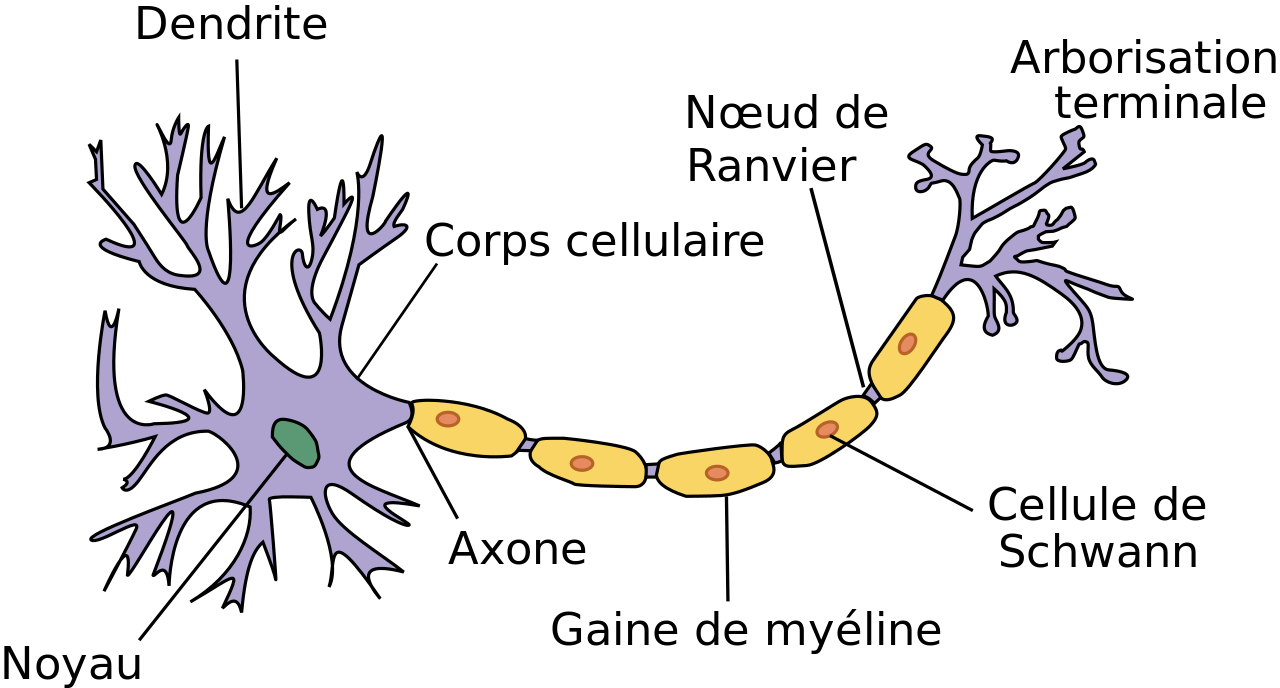
\includegraphics[width=8cm, height=3.5cm]{neurone.png}
	\caption{Aperçu d'un neurone multipolaire}
	\label{fig:neurone}
\end{figure}

La membrane cellulaire des neurones joue un rôle important dans la propagation des potentiels d'action, puisqu'elle est responsable de la régularisation de la différence de potentiel entre l'intérieur et l'extérieur de la cellule. Cette régularisation est effectuée par des pompes ioniques fixées sur la membrane qui permettent le transport d'ions Na et K. Ces structures utilisent l'ATP comme source d'énergie pour engendrer une différence de potentiel et créer un courant transmembranaire positif ou négatif, dépendemmant de la circonstance, responsable entre autre de rééquilibrer le système suite à une perturbation par un influx nerveux.


\subsection{Modélisation physique}

Le comportement d'un potentiel d'action se propageant à travers une neurone est décrit par le modèle électromagnétique complet. En se concentrant plus spécifiquement sur une dendrite, il est possible de réduire le problème à celui d'un courant voyageant à travers un conducteur à géométrie cylindrique. Par contre, plusieurs propriétés du neurone doivent être prises en considération puisqu'elles affectent le comportement du courant qui y circule. On sait, par exemple, dû à la nature des conducteur, que le milieu intracellulaire et extracellulaire posséderont une résistance quelconque. De plus, puisque les milieux interne et externe fortement conducteurs du neurone sont séparés par une membrane cellulaire peu conductrice, la membrane possédera une capacitance. Ces considérations sont traduites en un circuit éléctrique équivalent à la figure \ref{fig:membrane} qui représente une unité de longueur du neurone.

\begin{figure}[H]
	\centering
	\begin{circuitikz}
		\draw (0,0)
		to[short] (0,1)
		to[short] (-1,1)
		to[R=$r_m$] (-1,3)
		to[short] (1,3)
		to[C=$c_m$] (1,1)
		to[short] (0,1);
		
		\draw (0,3)
		to[short] (0,4)
		to[short] (1,4)
		to[R=$r_e$] (3,4)
		to[short] (4,4)
		to[short] (4,3)
		to[short] (3,3)
		to[R=$r_m$] (3,1)
		to[short] (5,1)
		to[C=$c_m$] (5,3)
		to[short] (4,3);
		
		\draw (4,1)
		to[short] (4,0)
		to[short] (3,0)
		to[R=$r_i$] (1,0)
		to[short] (0,0);
		
		\draw (0,0)
		to[short] (-1,0);
		
		\draw (0,4)
		to[short] (-1,4);
		
		\draw (4,4)
		to[short] (5,4);
		
		\draw (4,0)
		to[short] (5,0);
	\end{circuitikz}
	\caption{Circuit simulant les propriétés de la  membrane cellulaire d'un neurone. Les indices $e$ et $i$ dénottent respectivement l'extérieur et l'intérieur du neurone, tandis que l'indice $m$ dénote la membrane cellulaire.}
	\label{fig:membrane}
\end{figure}

Il est ensuite possible d'établir les équations (\ref{eq:i_m1}) et (\ref{eq:i_m2}) à partir du circuit. La première représente le courant transmembranaire, soit la somme des courants qui passe par la résistance et le condensateur, et la deuxième représente le courant voyageant parallèlement à la membrane du neurone.

\begin{equation}
\label{eq:i_m1}
i_m = i_c + i_r = c_m \frac{dV}{dt} + \frac{V}{r_m}
\end{equation}

\begin{equation}
\label{eq:i_m2}
i = \frac{1}{r_i + r_e} \frac{d^2V}{d^2x}
\end{equation}

Finalement, on suppose l'égalité entre (\ref{eq:i_m1}) et (\ref{eq:i_m2}). Le résultat, suite à quelques manipulations algébriques, est l'équation du câble (\ref{eq:cable}). Les solutions à cette équation différentielle sont connues et prennent la forme (\ref{eq:solution_cable}). La théorie prédit donc la propagation d'une onde plane atténuée exponentiellement en fonction de la distance parcourue.

\begin{equation}
	\label{eq:cable}
	\tau \frac{\partial V(x,t)}{\partial t} = \lambda^2\frac{\partial^2V(x,t)}{\partial x^2} - V(x,t), \hspace{1cm} \tau = r_mc_m, \  \lambda^2=\frac{r_m}{r_i+r_e}
\end{equation}

\begin{equation}
\label{eq:solution_cable}
	V(x,t) = \frac{e^{-kx}}{e^{\frac{-t}{\tau}}} sin(\omega t-kx), \hspace{1cm} k = \frac{1}{\lambda}\sqrt{\frac{1}{2}\omega \tau}
\end{equation}

Par contre, un problème émerge lorsque la solution à l'équation (\ref{eq:solution_cable}) est comparée avec des mesures expérimentales. Selon le modèle présenté, la différence de potentiel nécessaire à la génération d'influx nerveux serait de l'ordre de plusieurs milliers de volts! Une considération additionnelle doit être incluse dans le modèle; la présence des pompes ioniques dans la membrane cellulaire du neurone.


\subsection{Le modèle de Hodgkin-Huxley}\label{subsec:model}

En 1952, Alan Hodgkin et Andrew Huxley publient leur recherche sur la modélisation de la dyamique membranaire \cite{hodgkin_huxley}. Leur modèle consiste d'un système de quatre équations différentielles couplées de premier ordre (\ref{eq:dV_dt} - \ref{eq:dh_dt}), impliquant le potentiel transmembranaire (V ou $\phi$) ainsi que 3 fonctions-barrière \textit{n}, \textit{m} et \textit{h} qui définissent la probabilité d'activation des différentes pompes ioniques. Le modèle élimine la dépendance spatiale du potentiel et n'est donc valable que pour un point de l'espace. Les relations (\ref{eq:alpha_beta}) ont été déduites par Hodkin et Huxley à l'aide d'optimisations numériques basées sur des mesures expérimentales. Finalement, les valeurs des potentiels de repos $V_x$, des coefficients de conductance $g_x$ et de la capacitance membranaire $c_m$ sont incluses dans l'implémentation du modèle sur le dépôt GitHub \cite{github}.

\begin{align}
	\label{eq:dV_dt}
	\frac{dV}{dt} & = \frac{1}{c_m}( I_a - g_Kn^4(V - V_K) - g_{Na}m^3h(V - V_{Na}) - g_L(V - V_L)      )\\
	\label{eq:dn_dt}
 	\frac{dn}{dt} & = \alpha_n(V)(1-n) - \beta_n(V)n\\
 	\label{eq:dm_dt}
	\frac{dm}{dt} & = \alpha_m(V)(1-m) - \beta_m(V)m\\
	\label{eq:dh_dt}
	\frac{dh}{dt} & = \alpha_h(V)(1-h) - \beta_h(V)h
\end{align}

\begin{equation}
\begin{split}
\alpha_n (V) &= \frac{0.1-0.01V}{exp(1-0.1V) - 1}\\
\alpha_m (V) &= \frac{2.5-0.1V}{exp(2.5-0.1V) - 1}\\
\alpha_h (V) &= 0.07 exp(\frac{-V}{20})
\end{split}
\hspace{1cm}
\begin{split}
\beta_n (V) &= 0.125exp(\frac{-V}{80})\\
\beta_m (V) &= 4exp(\frac{-V}{18})\\
\beta_h (V) &= \frac{1}{exp(3-0.1V)+1}\\
\end{split}
\label{eq:alpha_beta}
\end{equation}

\section{Méthodologie}\label{sec:methodologie}

\subsection{Analyse numérique}\label{subsec:analyse}

Le modèle de Hodgkin-Huxley est solutionné numériquement en employant la méthode de Runge-Kutta d'ordre quatre. À partir de conditions initiales, l'algorithme construit itérativement une solution approximative aux équations différentielles ordinaires d'ordre un. La méthode débute par définir la discrétisation (\ref{eq:discretisation}) employant un pas de temps de longueur $h$ qui sépare les vecteurs solutions $u_n$.

\begin{equation}
t \rightarrow t_n,\hspace{1cm} t_{n+1} = t_n + h,\hspace{1cm} n = 0,1,2,...
\label{eq:discretisation}
\end{equation}

La méthode se base sur les séries de Taylor (\ref{eq:taylor}) pour estimer la solution au temps $t_{n+1}$ à l'aide de la solution au temps $t_{n}$. Une approche simpliste consiste à tronquer les termes d'ordre supérieur ou égal à deux, résultant en l'approximation (\ref{eq:approximation}), qui surestime les fonctions concaves et sous estime les fonctionc convexes.

\begin{equation}
	u(t+h) = u(t) + h \frac{du}{dt} + \frac{h^2}{2}\frac{d^2u}{dt^2} + \frac{h^3}{6}\frac{d^3u}{dt^3} + ... = \sum_{n=0}^{\infty} \frac{h^n}{n!}\frac{d^n}{dt^n}
	\label{eq:taylor}
\end{equation}

\begin{equation}
	u_{n+1} \approx u_n + h \frac{du}{dt}\rvert_{t_n}
	\label{eq:approximation}
\end{equation}

Une meilleur approximation peut être obtenue en utilisant la moyenne des pentes au temps $t_n$ et $t_{n+1}$. Puisque le vecteur solution $u_{n+1}$ est à priori inconnu, on l'estime avec (\ref{eq:approximation}). Il s'agit de la méthode de Heun (\ref{eq:heun}).

\begin{equation}
	u_{n+1} \approx u_n + \frac{h}{2}(\frac{du}{dt}\rvert_{t_n} + \frac{du}{dt}\rvert_{t_{n+1}})
	\label{eq:heun}
\end{equation}

Plusieurs autres techniques, tel que le pas adaptadif,  sont utilisées pour diminuer l'erreur. Elles sont explicitées dans le recueil de notes de Paul Charbonneau \cite{notes_cours}. L'implémentation de l'algorithme est incluse sur le dépôt GitHub \cite{github}.

\subsection{Mesures et simulations}\label{subsec:mesures_simulations}

D'abord, on confirme la calibration de l'algorithme en reproduisant quelques résultats démontrés dans le recueil de notes de Paul Charbonneau \cite{notes_cours}. Ces reproductions servent à démontrer que l'algorithme de Runge-Kutta est appliqué correctement sur le modèle de Hodgkin-Huxley et produit les résultats attendus. Ensuite, plusieurs mises en situation sont explorées, soient: 

\begin{enumerate}
	\item les courants continus;
	\item les courants en pulses;
	\item les courants à amplitude aléatoire;
	\item le coefficient de conductance $g_L$;
	\item la capacitance membranaire $c_m$;
\end{enumerate}

Dans le cas des courants continus, on cherche à décrire la relation entre la nature du courant appliqué et le comportement du modèle. À ces fins, on mesure l'effet de l'intensité du courant sur la fréquence et l'amplitude des potentiels d'action.  Ensuite, on s'intéresse au comportement du sytème lorsqu'il subit deux applications de courant séparées par une pause. Plus précisément, on cherche à comprendre les conditions requises afin de générer une double impulsion. On détermine donc la période de latence en fonction de l'intensité du courant. On explore par la suite les courants à amplitude aléatoire et l'épilepsie. On s'intéresse fondamentalement à décrire la réaction du système face à une perturbation aléatoire. Ensuite, on considère le coefficient de conductance $g_L$ qui nous permet de modéliser la sclérose en plaques. On cherche à décrire comment cette maladie réduit l'efficacité des neurones et leur sensibilité au courant appliqué. À ces fins, on détermine la valeur minimale que peut prendre $g_L$ avant d'observer une inhibition totale des influx nerveux en fonction de la grandeur et la durée du courant appliqué. Finalement, on s'intéresse au rôle de la capacitance membranaire $c_m$ et à son impact sur les potentiels d'action. On cherche une fois de plus une valeur critique avant l'inhibition des potentiels d'action. Par contre, il s'agit cette fois d'un maximum.

\section{Résultats et Discussion}\label{sec:resultats}

\subsection{Solution numérique du modèle de Hodgkin-Huxley}\label{sec:solution_numerique}

Le système d'équations différentielles présenté à la section \ref{subsec:model} est solutionné numériquement à l'aide de la méthode de Runge Kutta présentée à la section \ref{subsec:analyse}. Trois figures sont reproduites du manuel de cours \cite{notes_cours} à titre de comparaison. La figure \ref{fig:vnmh} simule un potentiel d'action et affiche la valeur des variables V, n, m et h en fonction du temps. Tel qu'attendu, on voit une période de croissance linéaire du potentiel durant l'application du courant, suivit d'une dépolarisation rapide qui atteind un maximum autour de 100 mV. On observe ensuite une période de repolarisation où le potentiel chutte. Finalement, le système se trouve en situation d'hyperpolarisation et revient lentement à l'équilibre. Les figures \ref{fig:tau} et \ref{fig:equil}, quant à eux, affichent respectivement le temps caractéristique des variables n, m et h et leur valeur à l'équilibre en fonction du potentiel.

\begin{figure}[H]
	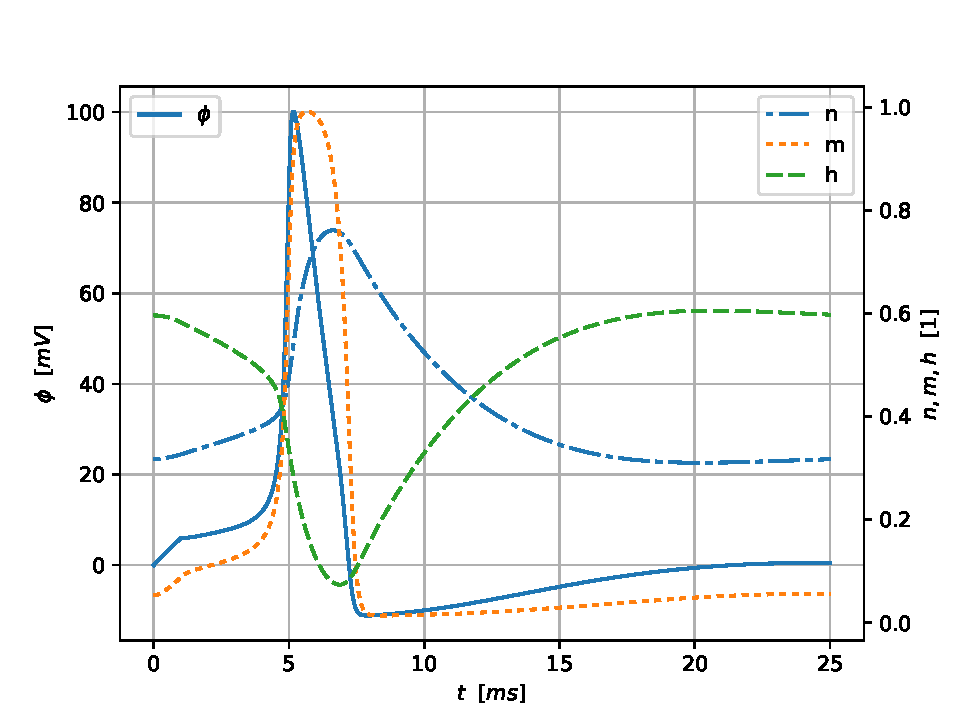
\includegraphics[width=6cm, height=6cm]{Vnmh.pdf}
	\centering
	\caption{Valeur des variables V, n, m et h en fonction du temps pour un potentiel d'action typique}
	\label{fig:vnmh}
\end{figure}

\begin{figure}[H]
	\begin{subfigure}{0.5\linewidth}
		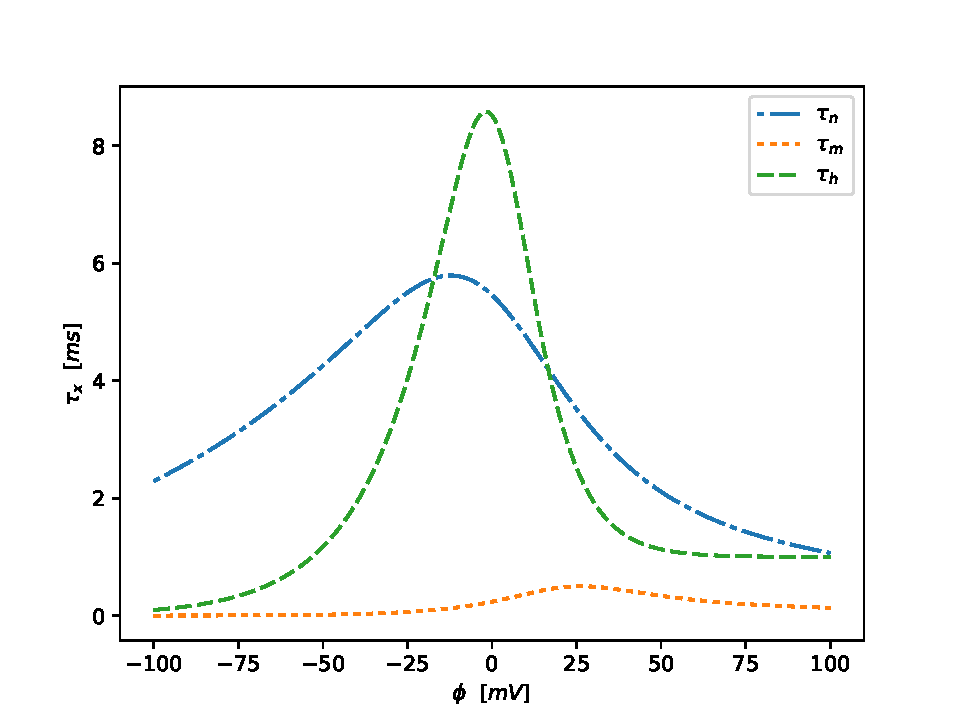
\includegraphics[width=6cm, height=6cm]{Tau.pdf}
		\centering
		\caption{Temps caractéristique des variables n, m et h en fonction de $\phi$ }
		\label{fig:tau}
	\end{subfigure}
	~
	\begin{subfigure}{0.5\linewidth}
		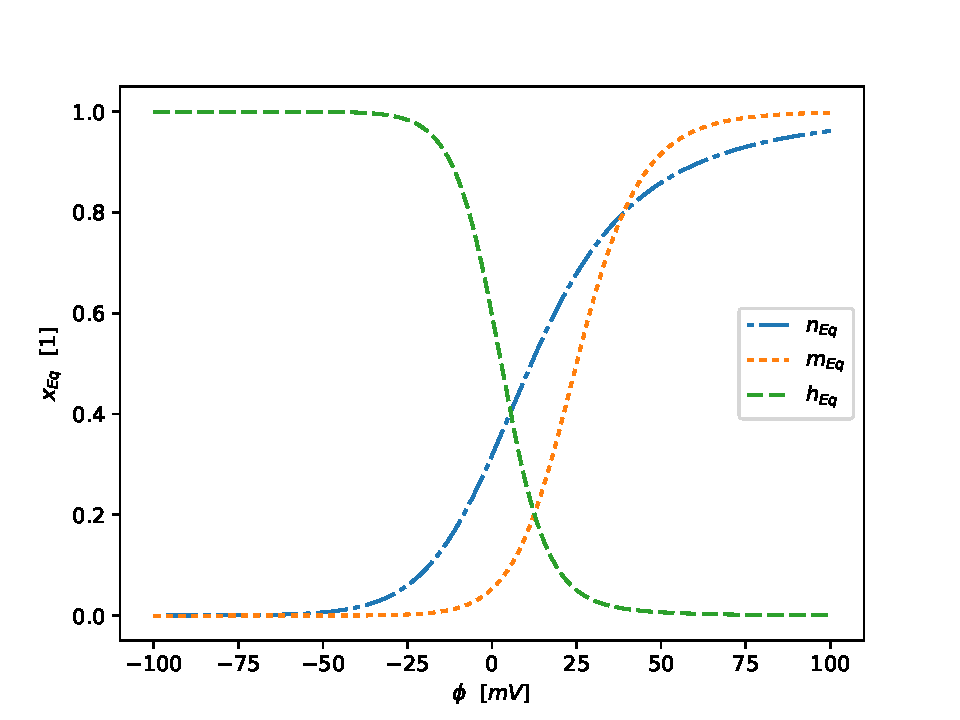
\includegraphics[width=6cm, height=6cm]{VarEquil.pdf}
		\centering
		\caption{Valeur à l'équilibre des variables n, m et l en fonction de $\phi$ }
		\label{fig:equil}
	\end{subfigure}
	\caption{Les propriétés des fonctions-barrière}
\end{figure}



\subsection{Application d'un courant continu}\label{sec:courant_continu}

À fins d'explorations initiales, on solutionne le modèle sous deux conditions différentes, soit une simulation avec un courant de $7 \mu A$ et la deuxième avec un courant de $10 \mu A$. La solution est présentée sur un intervalle de 80 ms à la figure \ref{fig:double_continuous}. On constate la présence d'une série de potentiel d'actions qui ne sont pas superimposés; l'intensité du courant transmembranaire influence la fréquence des impulsions. Plus précisément, on remarque que la fréquence augmente avec l'intensité du courant. De plus, on voit une déformation des impulsions due au courant continu en les comparant à l'impulsion simple de la figure \ref{fig:vnmh}. Finalement, on remarque que le premier potentiel d'action possède une amplitude légèrement supérieure à tous les autres, tandis que les autres ont une amplitude environ égale. À priori, il ne semble pas y avoir de différence d'amplitude entre le train de potentiels généré par le courant de $7 \mu A$ et celui de $10 \mu A$. 

\begin{figure}[H]
	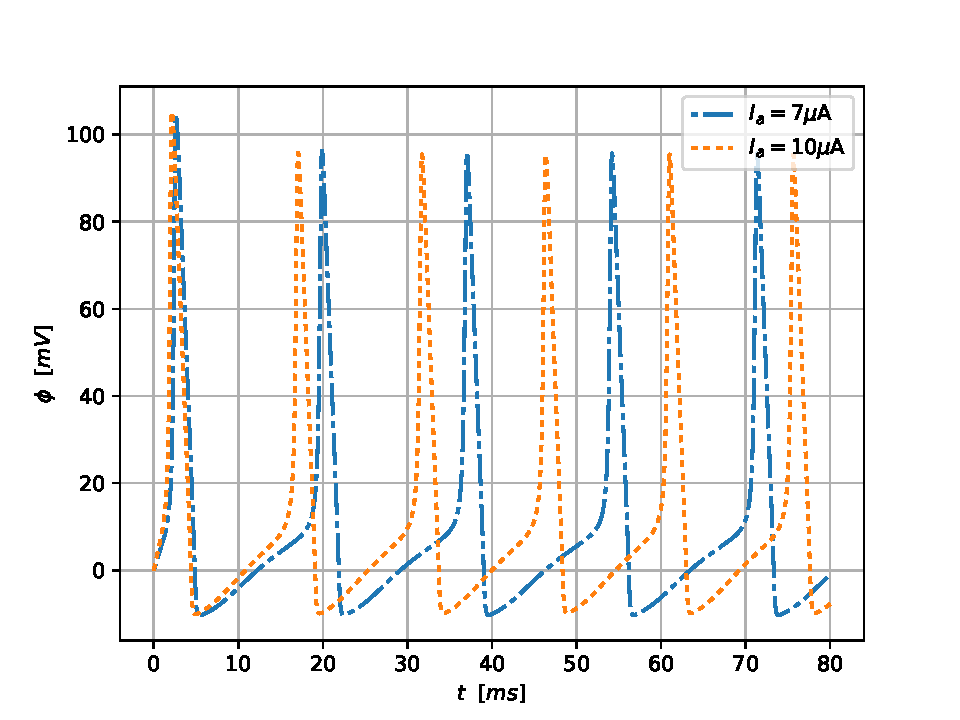
\includegraphics[width=6cm, height=6cm]{Potentiel_courant_continu.pdf}
	\centering
	\caption{Potentiel transmembranaire en fonction du temps pour des courants continus de $7\ et\ 10 \mu \  A$}
	\label{fig:double_continuous}
\end{figure}

On cherche maintenant à confirmer ou infirmer nos observations initiales. On se concentre d'abord sur la fréquence $f$ des oscillations de potentiel en fonction de l'intensité du courant. La fréquence est obtenue en mesurant la période $T$ des oscillations et en invoquant la relation $f=\frac{1}{T}$. Le premier potentiel d'action est ignoré dans l'analyse. En se référant à la figure \ref{fig:frequence}, on remarque que la dépendance observée plus tôt entre la fréquence et l'intensité du courant n'est pas linéaire mais demeure croissante sur l'intervalle observé.

On se concentre ensuite sur l'amplitude des oscillations de potentiel en fonction de l'intensité du courant transmembranaire. Les mesures sont effectués par rapport au point d'équilibre $V=0$ et le premier maximum est toujours ignoré. On remarque que notre observation initiale était erronée; l'amplitude des potentiels d'action dépend de l'intensité du courant. En se référant à la figure \ref{fig:amplitude}, on s'aperçoit que les courants de  $7 \mu A$ et  $10 \mu A$ utilisés durant l'analyse initiale généraient tous les deux des potentiels d'action avec des amplitudes similaires, causant une erreur d'interprétation.

\begin{figure}[H]
	\begin{subfigure}{0.5\linewidth}
	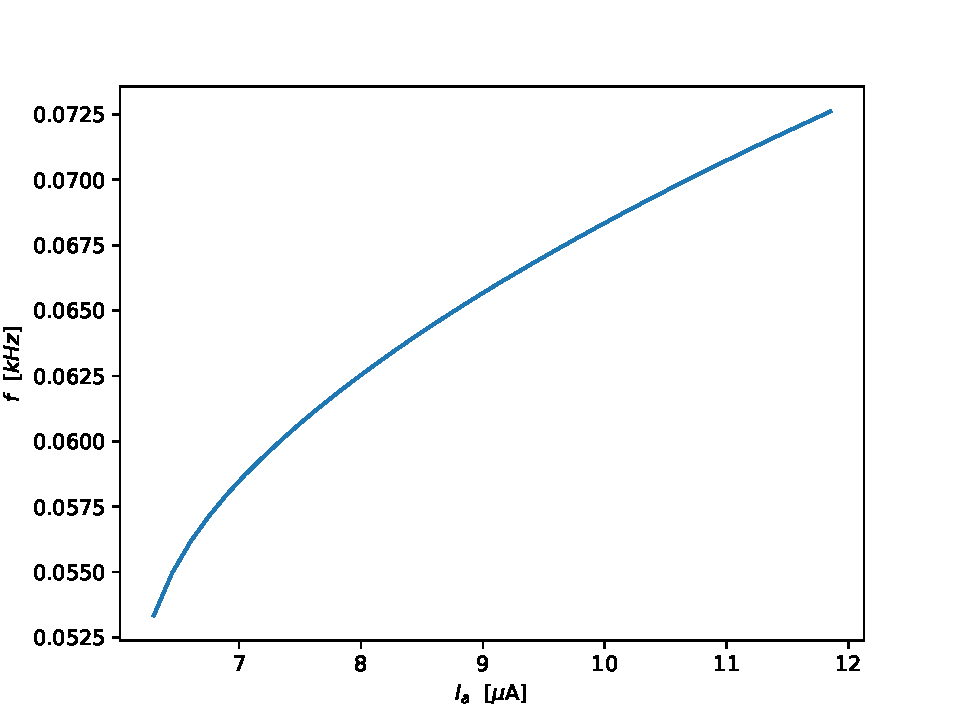
\includegraphics[width=6cm, height=6cm]{Frequency.pdf}
	\centering
	\caption{La fréquence des trains de potentiels en fonction de l'intensité du courant}
	\label{fig:frequence}
	\end{subfigure}
	~
	\begin{subfigure}{0.5\linewidth}
	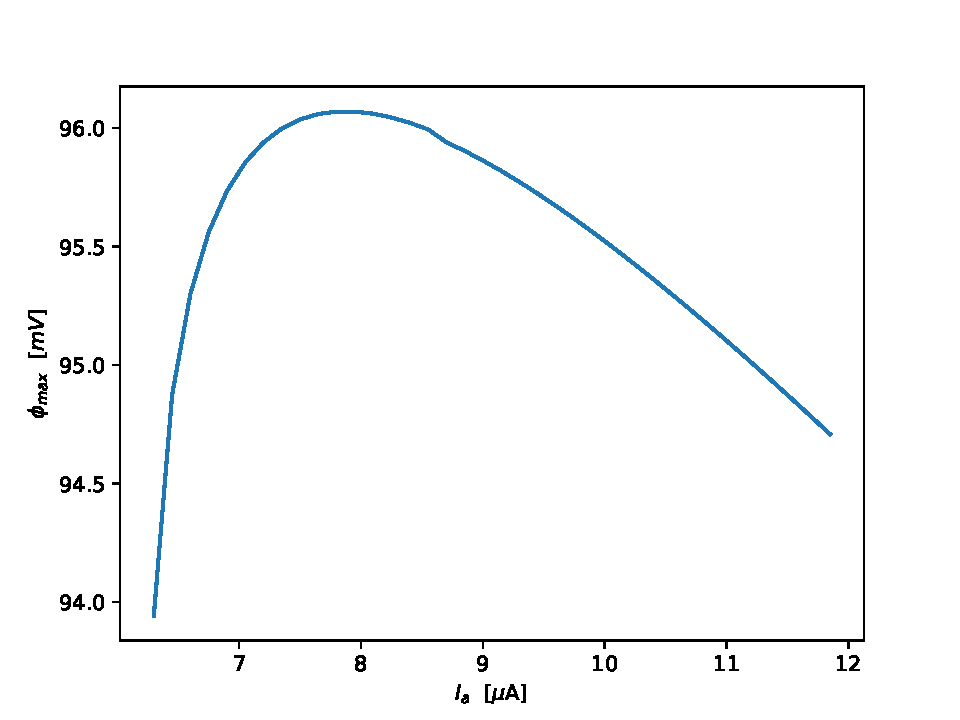
\includegraphics[width=6cm, height=6cm]{Amplitude.pdf}
	\centering
	\caption{L'amplitude moyenne des trains de potentiels en fonction de l'intensité du courant}
	\label{fig:amplitude}
	\end{subfigure}
	\caption{Analyse du comportement des trains de potentiels en fonction de la nature du courant appliqué}
	\label{fig:frequence_amplitude}
\end{figure}


\subsection{Application de courant en pulse}\label{sec:periode_latence}

On s'intéresse maintenant à la réaction du système lorsque soumis à des courants sur des intervalles discontinus. Plus précisément, on commence par explorer deux scénarios où un courant de  $7 \mu A$ est appliqué deux fois pendant $1ms$. La figure \ref{fig:double_echec} montre le résultat lorsque les applications sont séparées par une pause de 15 $ms$, tandis que la figure \ref{fig:double_succes} affiche le résultat pour pause de 20 $ms$. On remarque tout de suite une différence importante dans le comportement du modèle sous ces deux conditions; le nombre de potentiels d'action n'est pas le même. Si la deuxième application de courant apparaît trop top durant l'hyperpolarisation transitoire, la perturbation ne génère pas un deuxième potentiel d'action. On nomme cette borne minimale sur la différence de temps la période de latence $\Delta_{min}$. On cherche à caractériser davantage ce temps de latence.

\begin{figure}[H]
	\begin{subfigure}{0.5\linewidth}
		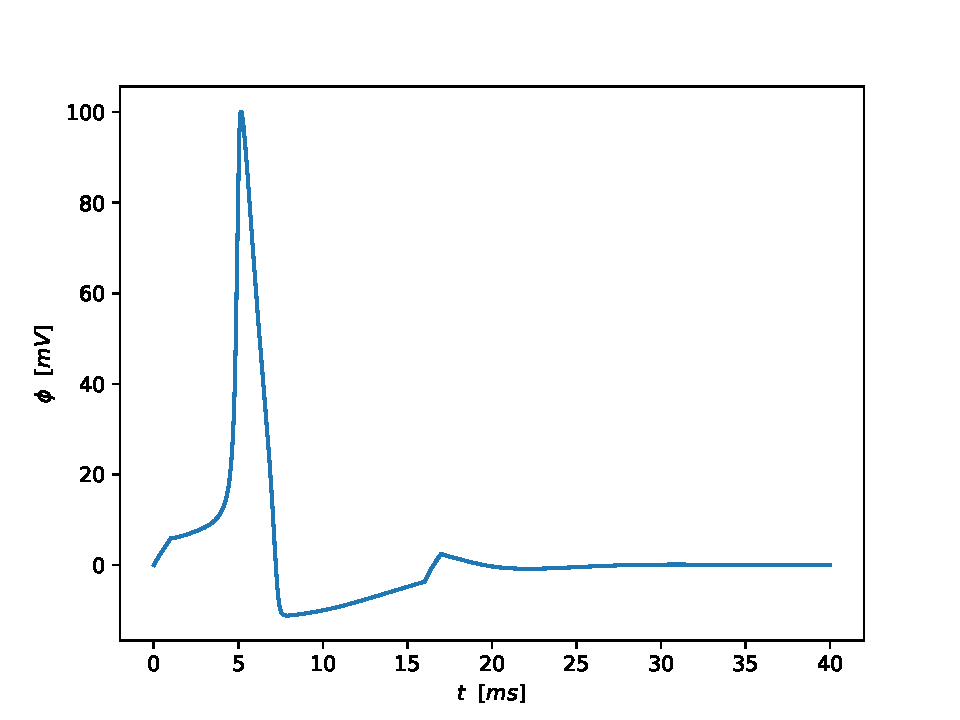
\includegraphics[width=5cm, height=5cm]{double_pulse_echec.pdf}
		\centering
		\caption{Applications d'un courant de $7 \mu A$ pendant $1\ ms$ séparées par une pause de $15\ ms$}
		\label{fig:double_echec}
	\end{subfigure}
	~
	\begin{subfigure}{0.5\linewidth}
		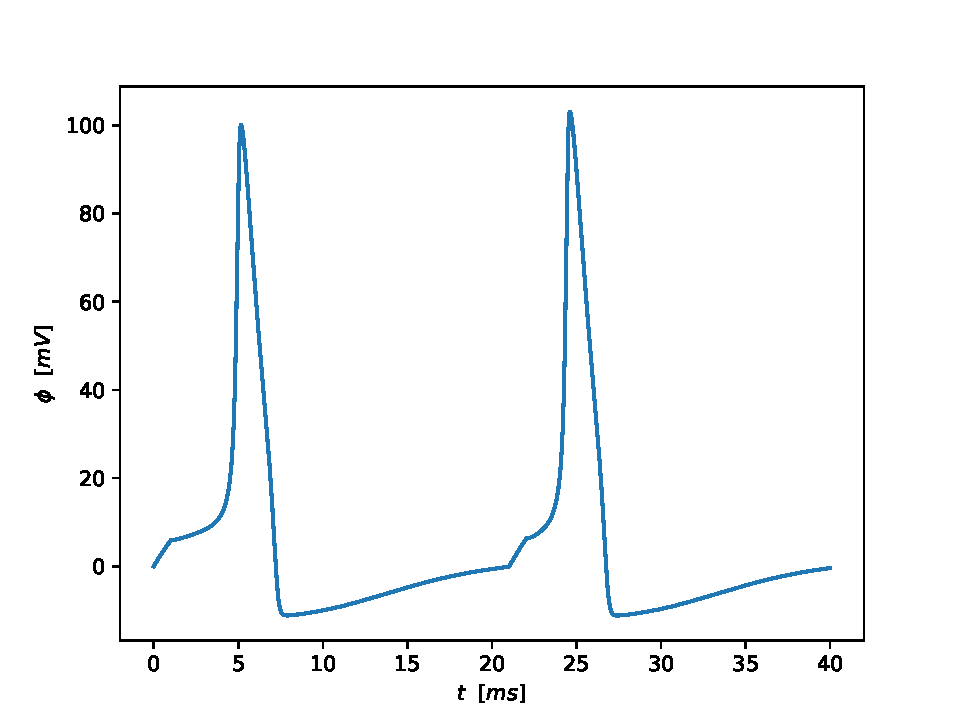
\includegraphics[width=5cm, height=5cm]{double_pulse_succes.pdf}
		\centering
		\caption{Applications d'un courant de $7 \mu A$ pendant $1\ ms$ séparées par une pause de $20\ ms$}
		\label{fig:double_succes}
	\end{subfigure}
	\caption{Exploration des conditions requises à l'observation d'une double impulsion}
	\label{fig:double_pulse}
\end{figure}

On évalue la période de latence sur un intervalle de courant de 7.5 à 24 $\mu A$. Un court algorithme  est développé \cite{github} pour approximer la valeur de $\Delta_{min}$ à chaque point de mesure. L'algorithme commence avec un $\Delta_{min}$ près de 0 et converge vers la solution en prenant des pas adaptatifs. L'erreur entre la sortie de l'algorithme et la valeur prédit par le modèle peut être choisie arbitrairement par le biais du paramètre $\epsilon$, mais impacte grandement le temps d'exécution de l'algorithme. Une erreur de $\epsilon = 2.5 \mu s$ est choisit comme compromis. La figure \ref{fig:min_delta} affiche la relation observée entre $\Delta_{min}$ et l'intensité du courant appliqué. On observe une décroissance de la période de latence lorsque l'intensité du courant augmente. Cette observation pourrait expliquer pourquoi les courants continus de plus forte intensité génèrent des potentiels d'action avec une fréquence plus élevée (voir figure \ref{fig:double_continuous}); le temps d'attente avant que le système redevienne susceptible est plus bas et donc plus d'impulsions sont générées par unité de temps. 

\begin{figure}[H]
	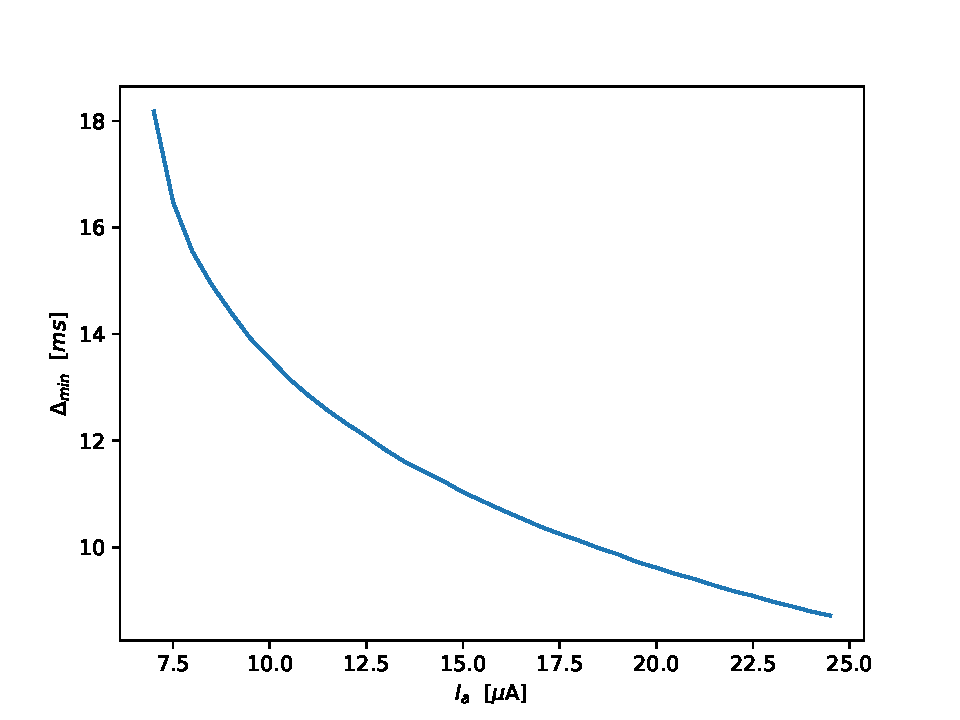
\includegraphics[width=5cm, height=5cm]{DeltaMinCurrent.pdf}
	\centering
	\caption{Temps minimal requis entre l'application de courants pour engendrer deux actions de potentiel}
	\label{fig:min_delta}
\end{figure}

Additionnellement, on considère la possibilité de la présence d'asymptotes. L'étude de l'asymptote verticale est peu concluante; en pratique, il s'agit simplement de l'amplitude de courant nécéessaire à la génération de potentiels d'action. Cette asymptote ce déplace donc en fonction de la durée d'application du courant. Si on s'intéresse plutôt au cas où $\Delta_{min} \rightarrow 0$, le courant appliqué doit rapidement augmenter pour compenser et cause une déformation des potentiels d'actions (voir la figure \ref{fig:small_delta}). On remarque aussi la diminution de l'amplitude de la deuxième impulsion. Ensemble, ces propriétés causent une ambiguité concernant la présence ou non d'une double impulsion. On se contente de remarquer que les conditions nécessaires pour atteindre de telles périodes de latence ne sont pas typiquement observées dans le cerveau humain. En toutes fins pratiques, le seuil inférieur de $\Delta_{min}$ dépend de l'intensité de courant maximale qui peut être appliquée sur le neurone par un agent extérieur.

\begin{figure}[H]
	\begin{subfigure}{0.5\linewidth}
		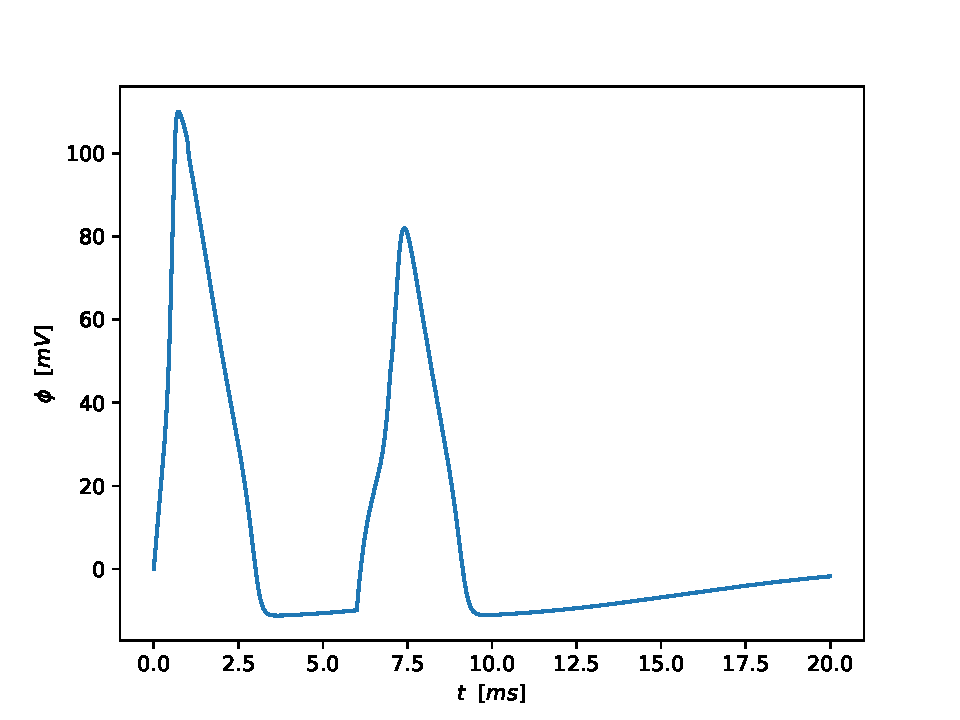
\includegraphics[width=5cm, height=5cm]{small_delta_100_5.pdf}
		\centering
		\caption{Potentiel en fonction du temps pour deux applications de courant de $100 \mu A$ de $1ms$ séparées par une pause de $5\ ms$}
		\label{fig:delta_100_5}
	\end{subfigure}
	~
	\begin{subfigure}{0.5\linewidth}
		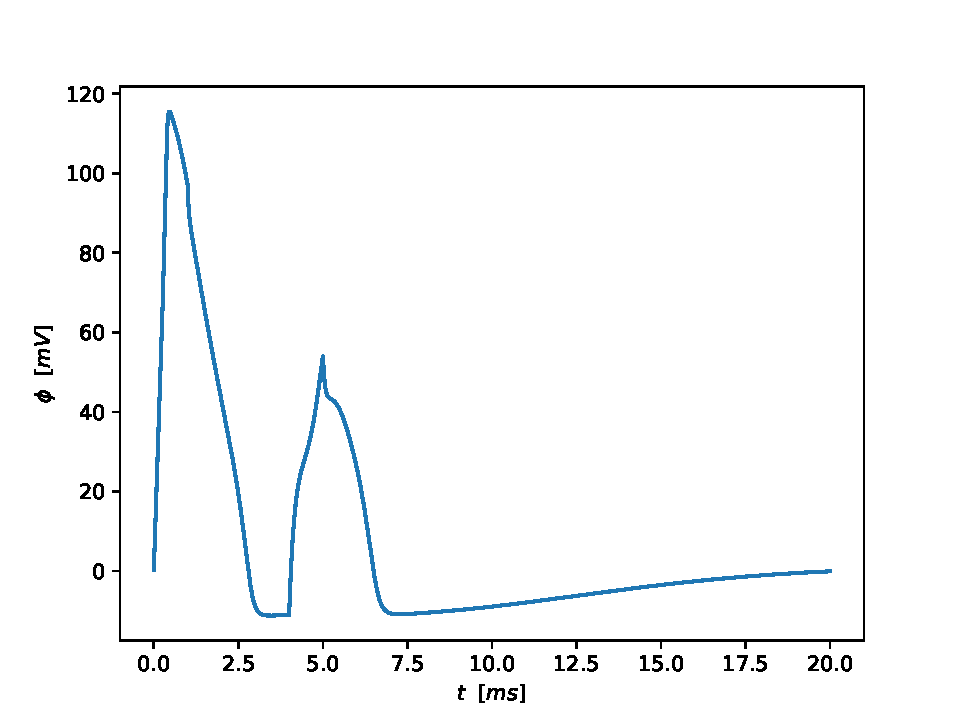
\includegraphics[width=5cm, height=5cm]{small_delta_250_3.pdf}
		\centering
		\caption{Potentiel en fonction du temps pour deux applications de courant de $250 \mu A$ de $1ms$ séparées par une pause de $3\ ms$}
		\label{fig:delta_250_3}
	\end{subfigure}
	\caption{Comportement du potentiel en fonction du temps lorsque $\Delta_{min} \rightarrow 0$}
	\label{fig:small_delta}
\end{figure}



\subsection{Courants à amplitude aléatoire}\label{sec:courant_aleatoire}

On observe maintenant le comportement du modèle de Hodkin-Huxley lorsque sujet à un courant d'amplitude aléatoire. Les amplitudes sont pigées de distributions gaussiennes centrées en $\mu_{I_a}=0\ \mu A$  et d'écarts types de $\sigma_{I_a}= 1,\ 2,\ 3\ \mu A$ à toutes les $2\ ms$. Les solutions sont affichées à la figure \ref{fig:random}. En se concentrant particulièrement sur la figure \ref{fig:random_1}, on remarque le comportement chaotique du potentiel. On observe une perte de périodicité et une absence de potentiels d'action. Les différences de potentiels demeurent petites mais relativement significatives. Lorsqu'on augmente l'écart type à  $\mu_{I_a}=2\ \mu A$, on voit apparaître quelques potentiels d'action séparés par de faibles oscillations. Finalement, lorsqu'on augmente l'écart type à  $\mu_{I_a}=3\ \mu A$, les influx nerveux redeviennent plus nombreux et on observe un certain retour de périodicité, bien qu'un bruit de fond demeure entre les potentiels d'action.

On constate que le comportement aléatoire du courant se propage et est reflété dans le comportement du potentiel. Même si la moyenne de l'intensité du courant est nulle, sa nature aléatoire signifie qu'elle peut être temporairement suffisament élevée pour déclencher un potentiel d'action. Cette variance génère un train de potentiels où l'amplitude de chaque potentiel d'action dépend de l'intensité du courant au moment du déclenchement. Une analyse supplémentaire est fournie à la section \ref{sec:capacitance_membranaire}, où on inclut une dimension additionnelle, soit la capacitance membranaire $c_m$.


\begin{figure}[H]
	\begin{subfigure}{0.5\linewidth}
		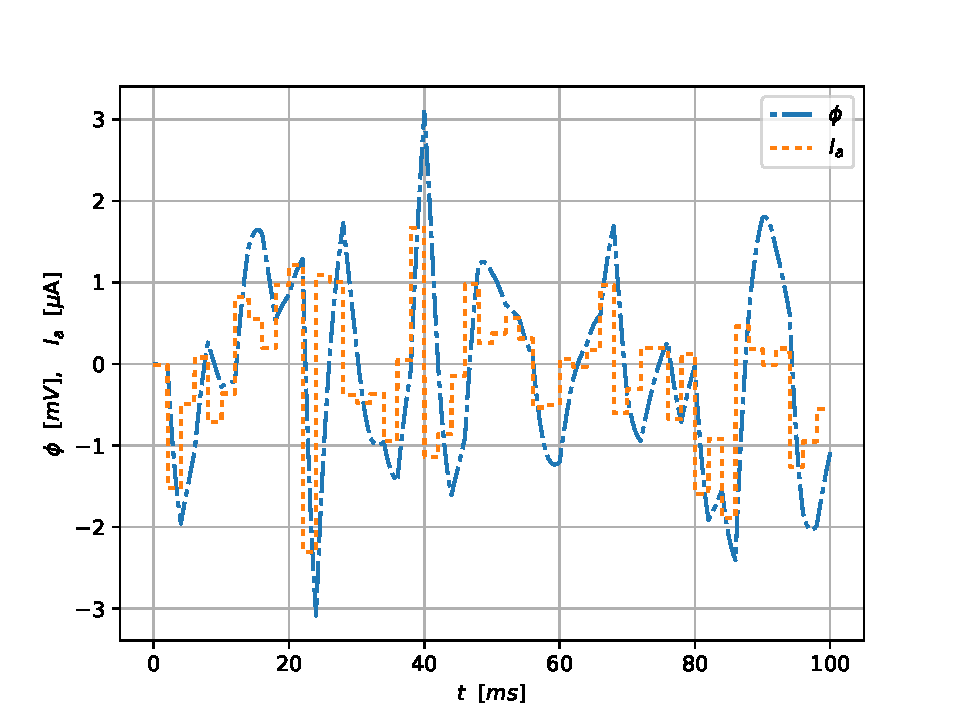
\includegraphics[width=5cm, height=5cm]{random_curr_1.pdf}
		\centering
		\caption{Amplitudes tirées d'une distribution gaussienne $N(\mu = 0, \sigma = 1)$}
		\label{fig:random_1}
	\end{subfigure}
	~
	\begin{subfigure}{0.5\linewidth}
		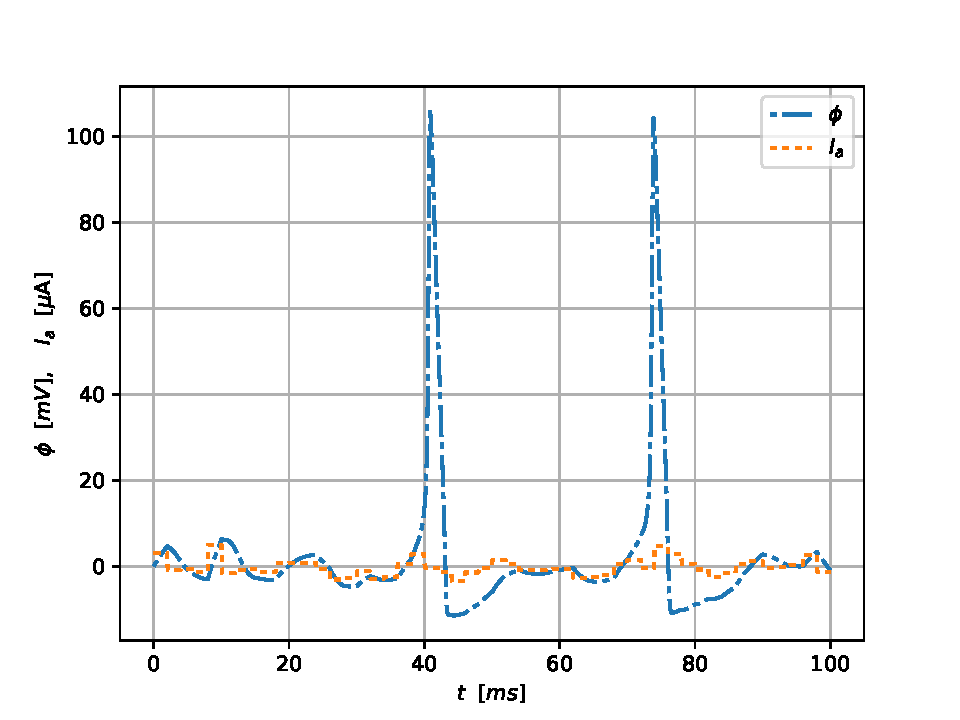
\includegraphics[width=5cm, height=5cm]{random_curr_2.pdf}
		\centering
		\caption{Amplitudes tirées d'une distribution gaussienne $N(\mu = 0, \sigma = 2)$}
		\label{fig:random_2}
	\end{subfigure}
	~
	\begin{center}
		\begin{subfigure}{0.5\linewidth}
		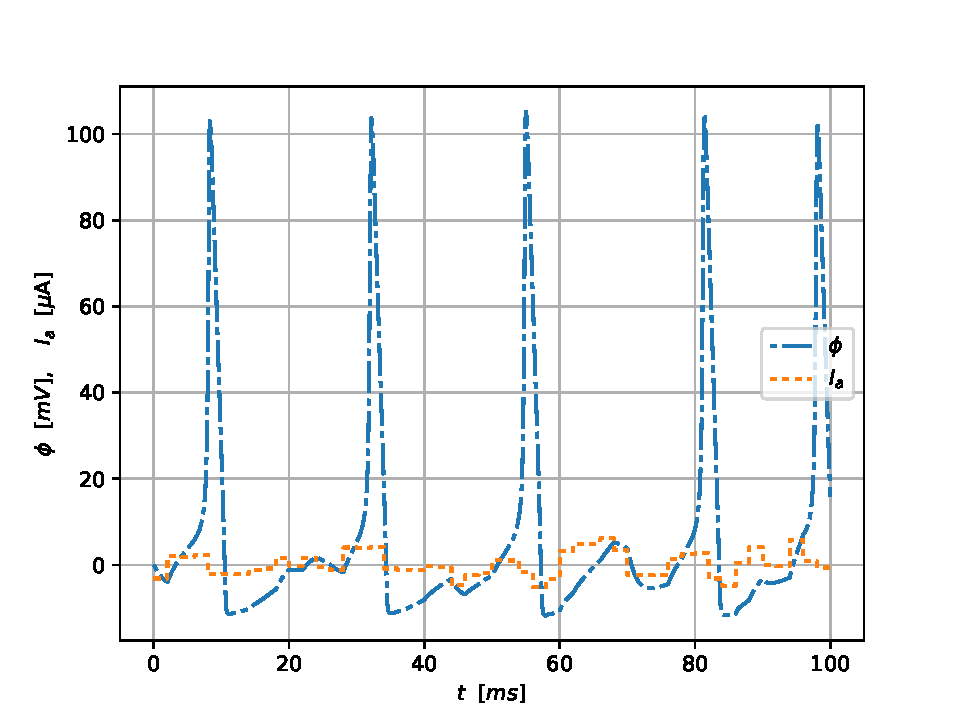
\includegraphics[width=5cm, height=5cm]{random_curr_3.pdf}
		\centering
		\caption{Amplitudes tirées d'une distribution gaussienne $N(\mu = 0, \sigma = 3$}
		\label{fig:random_3}
		\end{subfigure}
	\end{center}

	\caption{Applications de courants à amplitude aléatoire tirés de distributions gaussiennes. Lamplitude tu courant varie à toutes les 2 $ms$}
	\label{fig:random}
\end{figure}

\subsection{Le coefficient de conductance $g_L$}\label{sec:sclerose_plaque}

La sclérose en plaques est une maladie autoimmune qui engendre une détérioration des gaines de myéline situées sur l'axone. On peut reproduire cet effet en modifiant la valeur du coefficient de conductance $g_L$ dans l'équation (\ref{eq:dV_dt}). On cherche à voir l'effet qu'entraîne cette modification sur les trains de potentiels. Plus spécifiquement, on s'intéresse à la valeur minimale que peut prendre le coefficient $g_L$ avant que les potentiels d'actions soient complètement inhibés. On étudie la dépendance de ce phénomène avec l'intensité du courant et sa durée d'application. Un algorithme similaire à celui présenté à la section \ref{sec:periode_latence} est utilisé pour effectuer les mesures. Une erreur de $\epsilon = 5 \times 10^{-4} $  est choisie comme critère d'arrêt. Les sorties de l'algortithme sont affichées aux figures \ref{fig:gl_intensite} et \ref{fig:gl_length}. On remarque la comportement monotone décroissant des courbes sur leur intervalle. Cette décroissance se traduit par une perte de sensibilité des neurones au courant transmembranaire. Par exemple, chez une personne en santé avec un coefficient de conductance de $g_L = 0.3\ ms\ cm^{-2}$, un courant transmembranaire de  $7 \mu A$ appliqué pendant $1\ ms$ sera suffisant pour générer un influx nerveux, mais ce n'est nécéssairement pas le cas pour une persone atteinte de la sclérose en plaques. Un coefficient de $g_L = 0.29\ ms\ cm^{-2}$ serait suffisament bas pour inhiber les potentiels d'action qui seraient normalement présents lorsque $I_a = 7 \mu A$. On observe la même désensibilisation par rapport au temps d'application du courant transmembranaire; un temps d'application de 1.5 ms et une intensité de $5\ \mu A$ déclancherait un influx nerveux chez une personne normale, mais pas pour un coefficient inférieur à environ $25\ ms\ cm^{-2}$.

\begin{figure}[H]
	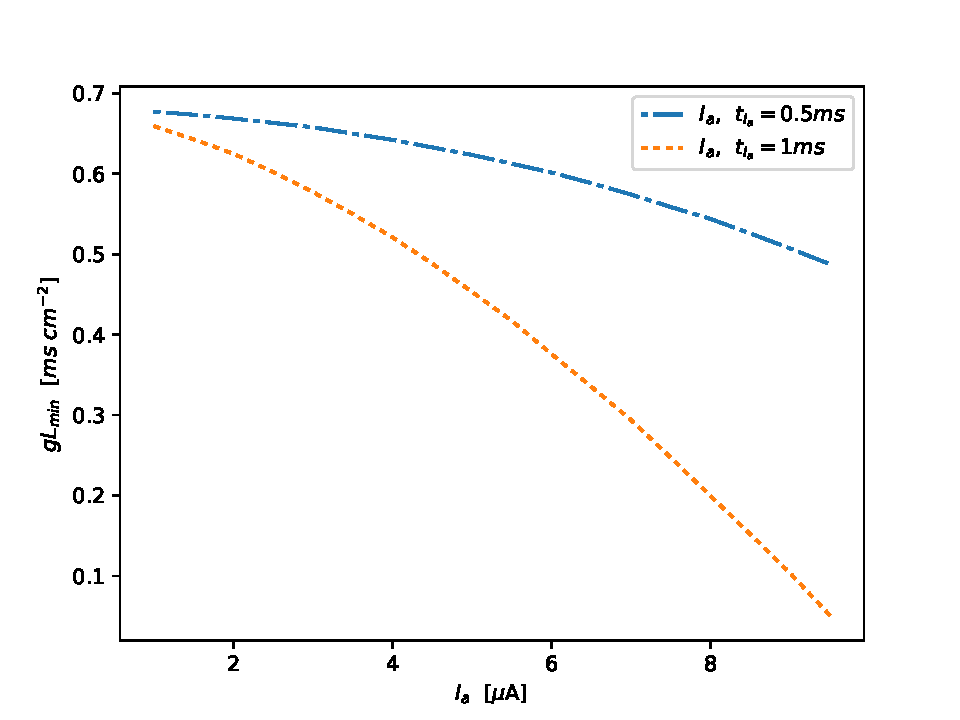
\includegraphics[width=6cm, height=6cm]{MingLAmperage.pdf}
	\centering
	\caption{Coefficient de conductance $g_L$ minimale  nécessaire au déclenchement d'un potentiel d'action en fonction de l'intensité du courant appliqué}
	\label{fig:gl_intensite}
\end{figure}

\begin{figure}[H]
	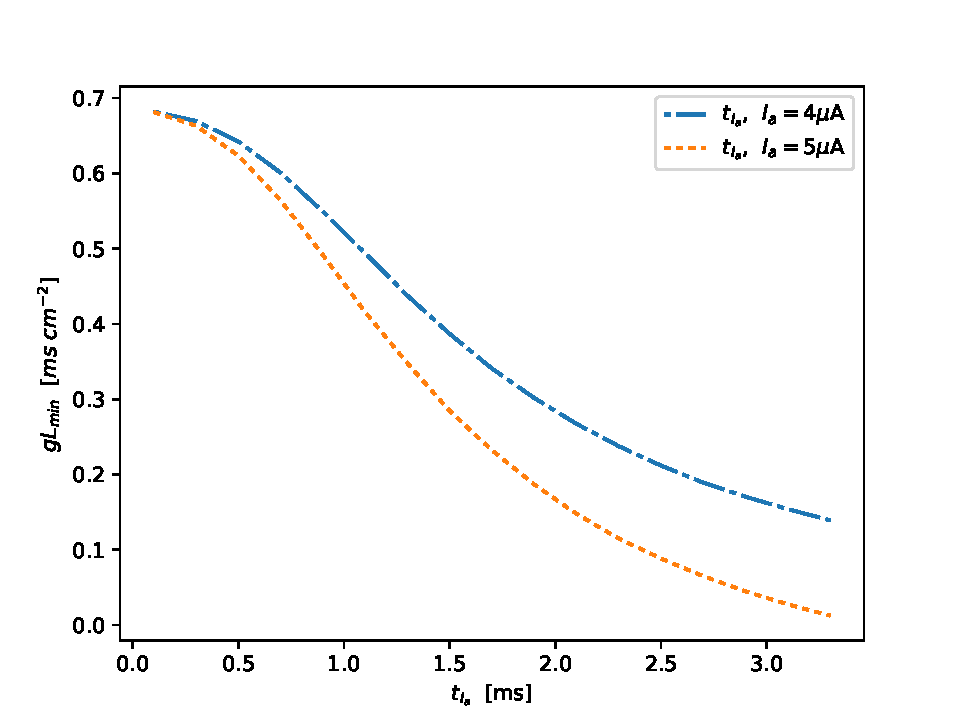
\includegraphics[width=6cm, height=6cm]{MingLLength.pdf}
	\centering
	\caption{Coefficient de conductance $g_L$  minimale nécessaire au déclenchement d'un potentiel d'action en fonction du temps d'application du courant}
	\label{fig:gl_length}
\end{figure}


\subsection{La capacitance membranaire $c_m$}\label{sec:capacitance_membranaire}

Finalement, on s'intéresse au rôle que joue la capacitance membranaire dans la régularisation des potentiels d'action. On commence par simuler deux scénarios, tous deux avec une capacitance membranaire de $c_m = 2 \mu F$, mais l'un avec un courant de $7 \mu A$  et l'autre avec un courant de $14 \mu A$. Les solutions de ces simulations sont affichés à la figure \ref{fig:cm_2}. 

\begin{figure}[H]
	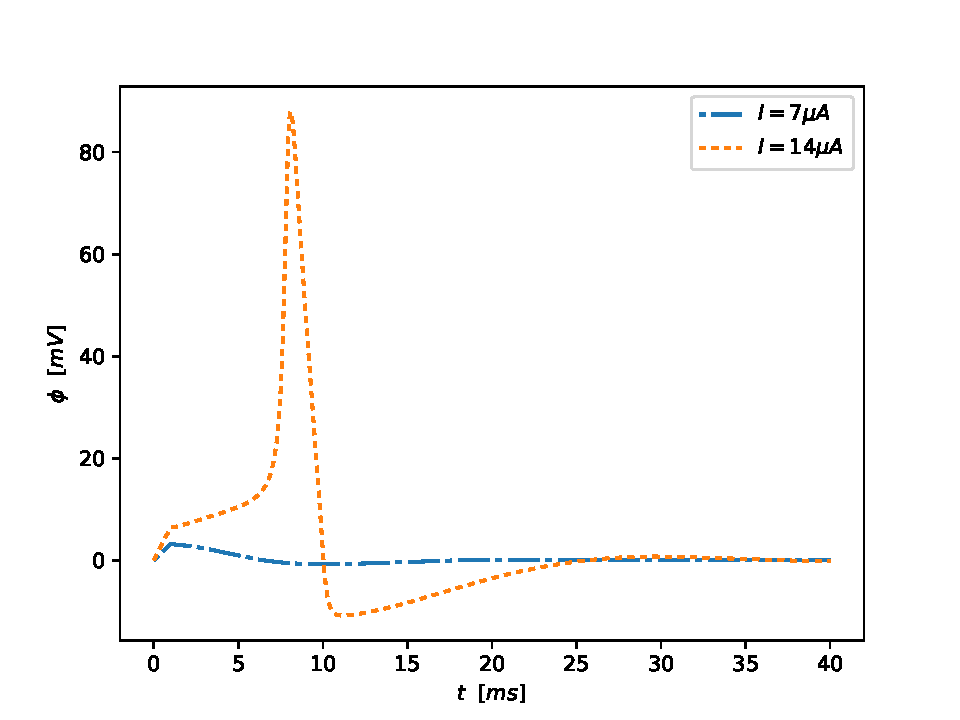
\includegraphics[width=6cm, height=6cm]{Cm_2.pdf}
	\centering
	\caption{Applications de courants de $7$ et $10\ \mu A$ pendant $1\ ms$ avec une capacitance membranaire de $c_m=2\ \mu F$}
	\label{fig:cm_2}
\end{figure}

On remarque d'abord l'asbence de potentiels d'action; l'augmentation de la capacitance cause une désensibilisation du système au courant transmembranaire. Inversément, une perte de capacitance membranaire engendrerait des déclenchements de potentiels d'actions qui auraient normalement été inhibés, ce qui soulève la question, une telle perte de capacitance engendre-t-elle une prédisposition aux crises d'épilepsie? Si on se réfère à la figure \ref{fig:random}, on remarque qu'un courant continu centré en 0 ne génère typiquement pas de potentiel d'action lorsque l'écart type est de 1, mais que c'est le cas lorsque l'écart type grandit. On lance une nouvelle simulation du courant aléatoire, mais cette fois-ci avec une capacitance membranaire de $C_m = 0.5$. La figure \ref{fig:random_cm} affiche la solution.

\begin{figure}[H]
	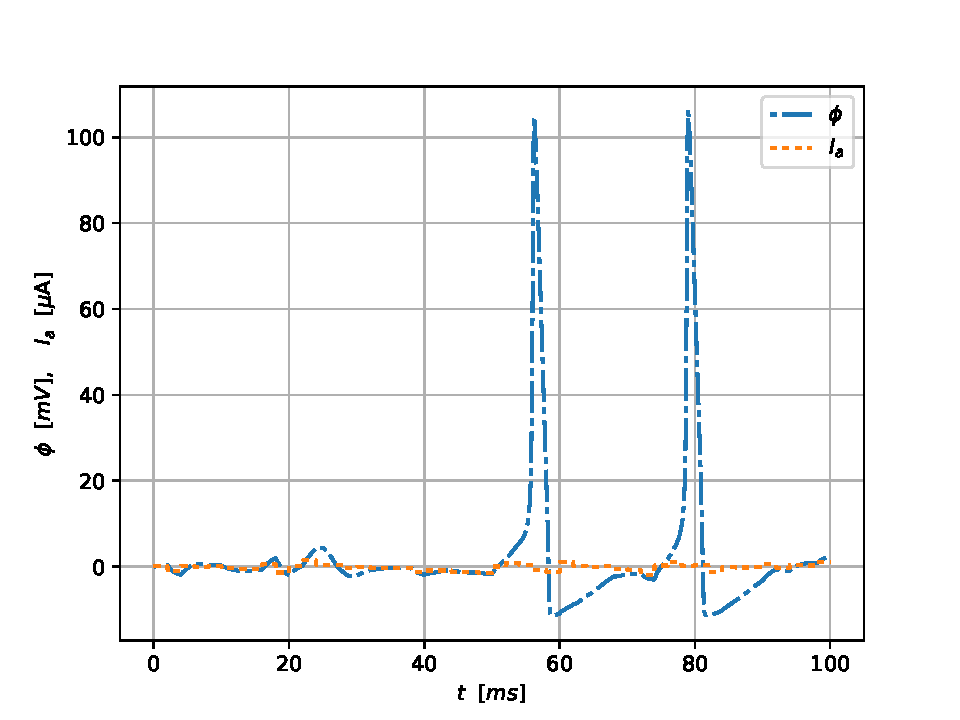
\includegraphics[width=6cm, height=6cm]{randomCm.pdf}
	\centering
	\caption{Application d'un courant continu à amplitude aléatoire. L'amplitude varie à toutes les $2\ ms$ et est obtenue à partir d'une gaussienne $N(\mu = 0, \sigma = 1)$. La capacitance membranaire est diminuée de moitier, soit $c_m=0.5\ \mu F$.}
	\label{fig:random_cm}
\end{figure}

On observe l'apparition de potentiels d'action, ce qui semble supporter notre hypothèse. Afin d'explorer davantage cette idée, on lance un nombre élevée de simulations basées sur la même distribution gaussienne mais avec des capacitances membranaires différentes et on compte le nombre de potentiels d'actions présents en moyenne. Les résultats sont affichés au tableau \ref{tab:nbinflux_cm} et viennent supporter l'hypothèse qu'une diminution de la capacitance membranaire augmente la sensibilité du neurone aux courants d'amplitudes aléatoires. 

\begin{table}[H]
	\centering
	\begin{tabular}{|c|c|c|}
		\hline
		 Nombres de simulations & Nombres de maxima, $c_m=0.5$ & Nombres de maxima, $c_m=1$\\\hline
		20 & 1.1 & 0.05 \\\hline
		50 & 1.2 & 0.06 \\\hline
		100 & 1.03 & 0.1 \\\hline
	\end{tabular}
	\caption{Nombre moyen de potentiels d'action en fonction de la capacitance membranaire $c_m$ pour un courant d'amplitude aléatoire suivant une distribution gaussienne $N(\mu = 0, \sigma = 1)$ appliqué pendant 80 ms.}
	\label{tab:nbinflux_cm}
\end{table}

Additionnellement, on mesure la relation entre la valeur maximale de $c_m$ pour laquelle les potentiels d'actions ne sont pas inhibiés et l'intensité du courant. La solution est affichée à la figure \ref{fig:max_cm} et prend une tendance pratiquement linéaire sur l'intervalle observé. 


\begin{figure}[H]
	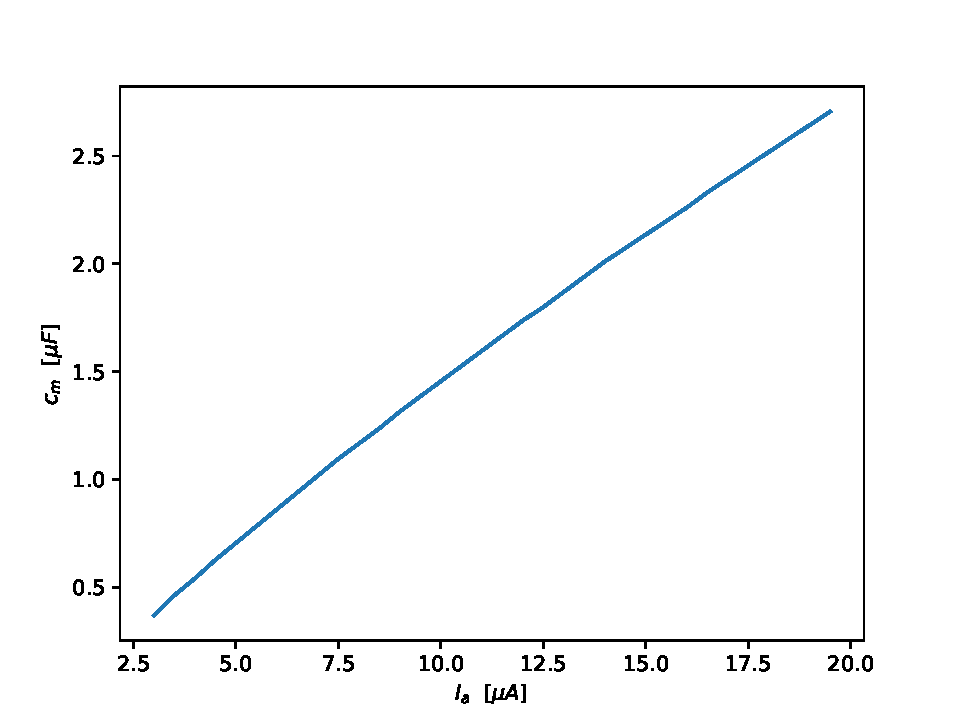
\includegraphics[width=6cm, height=6cm]{MaxCm.pdf}
	\centering
	\caption{Valeur maximale que peut prendre $c_m$ avant l'inhibition des potentiels d'action en fonction de l'intensité du courant}
	\label{fig:max_cm}
\end{figure}

\section{Conclusion}\label{sec:conclusion}

En utilisant une méthode de résolution numérique des équations différentielles ordinaires de premier ordre, soit la méthode de Runge Kutta d'ordre quatre, il a été possible d'explorer le modèle de Hodgkin-Huxley qui décrit la dynamique membranaire des neurones. En simulant l'application  d'un courant continu, il a été possible de décrire le comportement de la fréquence et de l'amplitude des potentiels d'action en fonction de l'intensité du courant. Ensuite, en appliquant deux courants successivement et en variant la pause entre les deux applications, il a été possible d'étudier la période de latence du système, qui diminue non linéairement avec l'intensité du courant. De plus, les courants à amplitude aléatoire ont permi d'explorer des comportements plus chaotiques se rapprochant des crises d'épilepsie. Finalement, l'effet du coefficient de conductance $g_L$ et de la capacitance membranaire $c_m$ sur les potentiels d'action ont été explorés en trouvant des seuils critiques qui déterminent si un influx nerveux sera généré ou inhibé. 

\pagebreak

\section{Bibliographie}\label{sec:bibliographie}
\begin{thebibliography}{l}
	\bibitem{notes_cours} 
	\textsc{Charbonneau}, P., Recueil de notes, Modélisation numérique en physique, Département de Physique, Université de Montréal, Janvier 2019
	
	\bibitem{hodgkin_huxley} 
	\textsc{Hodgkin}, A.L., \& Huxley, A., J. Physiology, 117(4), 500, 544 (1952)
	
	\bibitem{github}
	\textsc{Pfleiderer}, E., Dépôt GitHub, https://github.com/EricPfleiderer/Portfolio/tree/master/PHY3075/PROJET1
\end{thebibliography}

	
\end{document}